\chapter[Функции pyGrav]{Функции pyGrav}
\label{chap:pygrav_functions}

Этот раздел является фактическим руководством по использованию программы,
описывающим функции и технические характеристики. Программа запускается с
единственной доступной опцией <<Start project>> в меню <<File>>. Пользователю
предлагается указать папку ввода, в которой должны храниться все входные данные,
и папку вывода, которая будет использоваться программой для записи выходных
файлов.

\begin{figure}[h]
    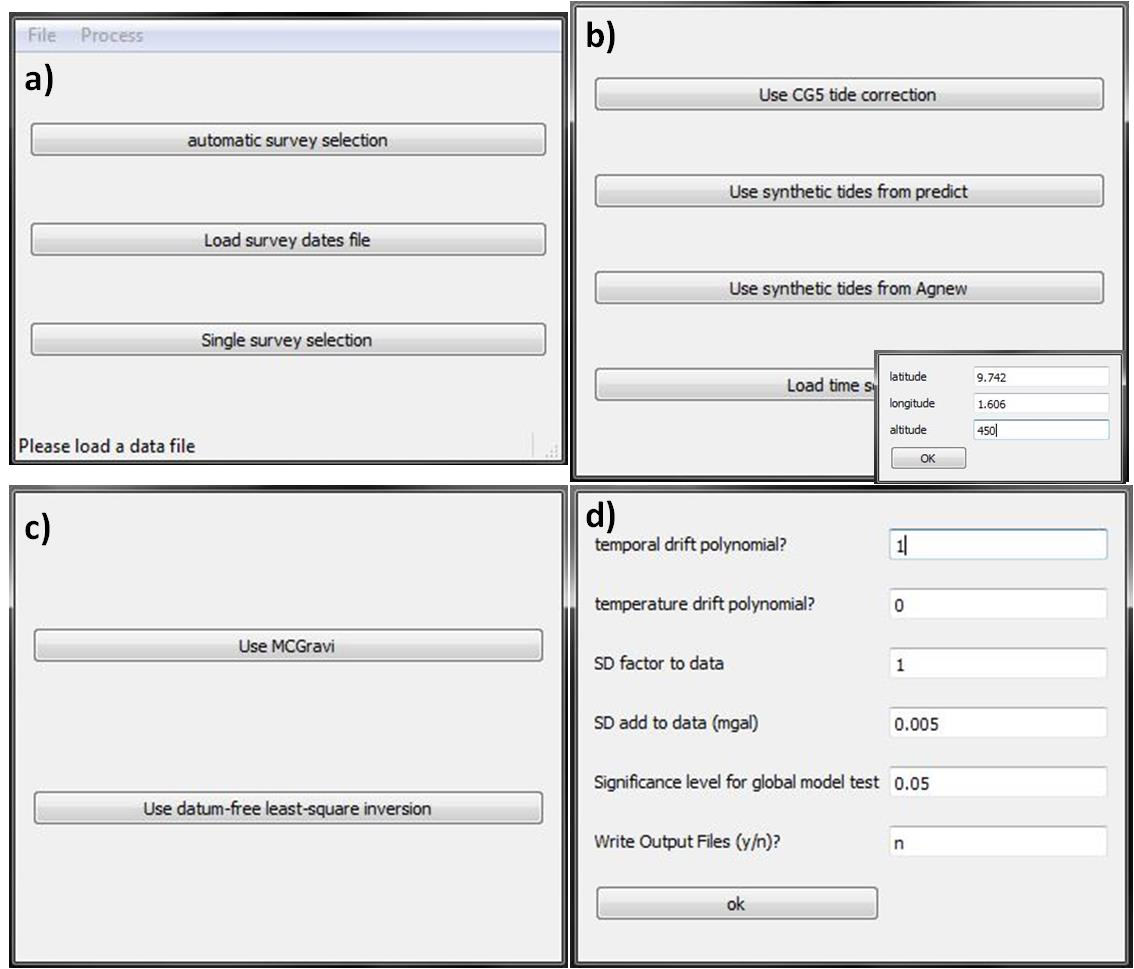
\includegraphics[width=\textwidth]{figures/example_of_pygrav_snapshots}
    \caption{Пример снимков \pg{}: a) Экран загрузки данных, b) Экран поправок
    за прилив, c) Экран компенсации сети и d) параметры компенсации сети.}
    \label{fig:example_of_pygrav_snapshots}
\end{figure}

\section[Загрузка данных]{Загрузка данных}
\label{sec:loading_data}

Доступны два варианта. Для продолжения/изменения обработки данных можно
загрузить <<raw data>> или <<processed data>>. При выборе <<processed data>>,
данные уже отсортированы в соответствии с иерархией съёмка/петля/пункты, в то
время как для <<raw data>> должны быть отсортированы. Таким образом, этот шаг не
только загружает данные, но и сохраняет их в соответствии с их иерархией (съёмки
-- петли -- пункты).

\subsection[Загрузка необработанных данных]{Загрузка необработанных данных}
\label{subsec:loading_raw_data}

Для выбора необработанных данных доступно три варианта:
\begin{itemize}
    \item Автоматический выбор съемки: для простой геометрии съемки, когда
    базовая станция всегда одна и та же, эта опция позволяет автоматически
    определять различные съемки на основе простого временного порога,
    запрошенного программой: выделяются разные съемки, если время между двумя
    последовательными сменами станций превышает пороговое значение. Если базовая
    станция и станция петли -- одни и те же, но имеют разные названия,
    следует выбрать параметр 0.

    \item Загрузка из файла даты начала/окончания съемки: эта опция позволяет
    считывать только съемки, определенные между датами начала и окончания,
    указанными во входном файле. Формат такого входного файла следующий:

    \begin{verbatim}
2012/07/11 05:17:00 2012/07/11 13:00:00
2012/07/13 05:00:00 2012/07/13 22:00:00
...
    \end{verbatim}
    
    \item Ручной ввод дату начала/окончания одной съемки (выбор единичной 
    съёмки)
    
\end{itemize}

Затем, петли в съёмках идентифицируются следующим образом: каждый раз,
когда обнаруживается базовая станция, запускается новый цикл, а предыдущий
завершается. Однако в более поздней процедуре корректировки дрейфа
обрабатываются вложенные петли, поскольку каждый цикл является частью одной и
той же системы уравнений, которая инвертируется с использованием метода
наименьших квадратов.

\subsection[Загрузка обработанных данных]{Загрузка обработанных данных}
\label{subsec:loading_processed_data}

Это эквивалентно загрузке <<project>>. Это позволяет повторно загрузить уже
обработанные данные. Данные должны быть предварительно сохранены с помощью
<<Save processed data>>, что, эквивалентно сохранению <<project>>, или
упорядочены требуемым образом. Пользователю предлагается загрузить файл,
описывающий иерархию данных. Формат такого файла следующий:

\begin{verbatim}
Directory C:/Users/…/test_case/output_data/
Survey: 2013-09-19 nloops: 4 directory: 2013-09-19
Loop: 1 filename: fn111c13.262.txt
Loop: 2 filename: fn211c13.262.txt
Survey: 2013-09-21 nloops: 4 directory: 2013-09-21
Loop: 1 filename: fn111c13.264.txt
Loop: 2 filename: fn211c13.264.txt
Loop: 3 filename: fn311c13.264.txt
Survey: ...
Loop: ...
\end{verbatim}

Строки <<Survey>> описывают доступные съёмки, названия съёмок (дата первого
измерения), количество петель, присутствующих в съёмках, и названия папок
съёмок в корневом каталоге. Строки <<Loop>> описывают для каждой строки в каждой
съёмке название петли и файл данных петли. Файлы данных похожи на файлы CGxTool
‘c’, но без заголовка и дополнительного столбца, содержащего статус данных (1
или 0, независимо от того, сохранена строка данных для корректировки дрейфа или
нет).

\section[Поправки данных]{Поправки данных}
\label{sec:data_corrections}

\subsection[Земные приливы]{Земные приливы}
\label{subsec:earth_tides}

Доступны четыре варианта коррекции приливов:
\begin{itemize}
    \item Используйте коррекцию прилива CG5 (ничего не делайте): Географические
    координаты должны быть введены в прибор до начала съемки.

    \item Используйте синтетические приливы из predict: Для пользователей window
    функция PREDICT из программного пакета ETERNA \cite{wenzel_1996} подключается к
    программе (см. раздел 8 об установке) для создания синтетического прилива на
    основе параметров tidal, который используется в качестве коррекции. Выбор
    приливного потенциала HW95 \cite{hartmann_hw95_1995} запрограммирован в
    pyGrav, но при необходимости его легко изменить. Параметры Tidal - это либо
    стандартные параметры tidal, либо вводимые пользователем в виде одного
    файла. Необходимо ввести географические координаты съемки.

    \begin{itemize}
        \item Экземпляр программы predict (.exe) должен быть доступен в папке с
        исходным кодом и копируется pyGrav в выходную папку, где производится
        вычисление.

        \item Стандартные параметры tidal считываются из файла (200D.INI) в
        папке основного кода

        \item формат файла параметров tidal, вводимого пользователем, должен
        быть следующим:

        \begin{verbatim}
0.023812    0.044652    1.13344    0.5445 MM
0.060132    0.080797    1.12607    -0.1195 MF
0.096423    0.249951    1.14548    0.6833 MTM
…
        \end{verbatim}
        (frq. начало полосы пропускания (cpd) – frq. конец bdwth (cpd) –
        амплитуда – фаза – название прилива)
        
    \end{itemize}

    \item Используйте синтетические приливы из Agnew: это негармонический метод,
    такой, который предусмотрен кодами fortran \cite{agnew_2007, agnew_2012} и позже
    переведен в MATLABTM \cite{cattin_gravprocess_2015} в их программе GravProcess. В
    данном случае поправка представляет собой прямое вычисление приливного
    потенциала по \cite{munk_tidal_1966}. Он основан на внутренних эфемеридах
    (для определения положения Луны и Солнца). Необходимо указать местоположение
    съемки.

    \item Загрузить временные ряды: если в качестве временных рядов доступен
    другой синтетический прилив, его можно загрузить и использовать в качестве
    коррекции. Принятый формат файлов - файлы ETERNAL или Tsoft (.TSF). Если
    расширение файла не .tsf, он будет рассматриваться как внешний файл. По
    умолчанию данные должны храниться в первом канале (столбце).
    
\end{itemize}

\subsection[Океаническая нагрузка]{Океаническая нагрузка}
\label{subsec:ocean_loading}

Загрузку океана можно скорректировать, используя два различных подхода:
\begin{itemize}
    \item Если анализ приливов может быть выполнен на месте съемки (например,
    благодаря близкому расположению сверхпроводящего гравиметра), можно перейти
    к коррекции земных приливов, используя PREDICT из пакета ETERNA (см. выше) и
    предоставляя параметры приливов из анализа приливов. Этот эмпирический
    подход учитывает как земные приливы, так и коррекцию нагрузки на океан (но
    может также учитывать другие воздействия окружающей среды, такие как
    давление воздуха, которые происходят с аналогичной частотой).
    
    \item Коррекция загрузки океана в программе pyGrav такая же, как и в коде
    процесса Grave \cite{cattin_gravprocess_2015}. Он основан на Agnew (2012) и на
    транскрипции MATLABTM от \cite{cattin_gravprocess_2015}. Коэффициенты загрузки океана
    должны быть загружены из отформатированного файла, предоставленного
    бесплатным поставщиком ocean компании Scherneck
    (http://holt.oso.chalmers.se/loading /). Параметры требуются для
    полусуточных (M2, S2, N2, K2), суточных (O1, P1, Q1, K1) и
    долгопериодических (MF, Mm, Ssa) приливных гармоник.
\end{itemize}

\subsection[Атмосфера]{Атмосфера}
\label{subsec:atmosphere}

Загрузите один временной ряд. Принятый формат файлов - файлы ETERNAL или Tsoft
(.TSF). Если расширение файла не .tsf, он будет рассматриваться как внешний
файл. По умолчанию данные должны храниться в первом канале (столбце).

\section[Выбор данных]{Выбор данных}
\label{sec:data_selection}

Это оригинальная функция программы. Иерархия данных видна в виде дерева, таблицы
и графического представления. Съемку, циклы, станции и единичные измерения можно
проверить или снять флажок, следует ли их сохранять для процесса корректировки
дрейфа (и окончательных простых расчетов разности). Это можно сделать либо
вручную, либо следуя автоматическим процедурам отбора, основанным на простых
пороговых критериях. В настоящее время к ним относятся 
\begin{itemize}
    \item пороговое значение для наклонов: абсолютные значения наклонов,
    превышающие входное значение, не отмечены
    
    \item пороговое значение стандартного отклонения силы тяжести (SD): значения
    SD, превышающие входные значения, не отмечены.

    \item пороговое значение, основанное на значениях силы тяжести: значения
    абсолютной силы тяжести, превышающие среднее значение трех последних
    значений + входное пороговое значение, не отмечены

    \item критерий длительности: если длительность данных отличается от входного
    значения, они не отмечаются. Это часто происходит, когда пользователь
    сохраняет текущие данные в поле при остановке сбора CG5.

\end{itemize}

Когда выбраны отдельные пороговые значения, они применяются только к текущей
таблице. При нажатии кнопки “применить ко всем данным” используются все входные
пороговые значения, причем для всего набора данных.

Другой вариант быстрой проверки/снятия флажков с данных - выделить несколько
строк с помощью мыши и нажать кнопки “проверить выбранное” или “снять флажок с
выбранного”.

Каждое обследование и циклы идентифицируются по датам их первых измерений.
Указаны номера станций, а число в скобках - это номер повторения, поскольку
некоторые станции повторяются (например, базовая станция). Данные организованы в
хронологическом порядке.

Ручной выбор может быть выполнен на основе табличных значений или графических
отображений, в зависимости от предпочтений пользователя. На графическом дисплее
непроверенные данные отображаются черным цветом, в то время как отмеченные
данные - синим. На экране гравитации среднее значение выбранных данных
отображается синей горизонтальной линией.

После выбора данных следует нажать кнопку OK. Это действие мало что дает, но
может быть важным: оно используется для проверки того, что на некоторых станциях
данные не выбраны, и в этом случае они удаляются. Это может произойти с помощью
автоматического выбора.

\section[Уравнивание дрейфа]{Уравнивание дрейфа}
\label{sec:drift_adjustment}

Как только поправки будут применены и данные выбраны, можно приступать к
корректировке дрейфа. Доступны два варианта. Можно запустить либо MCGravi
(Beilin, 2006) (если он установлен, см. раздел 8), либо использовать простую
схему инверсии наименьших квадратов без данных \cite{hwang_adjustment_2002}.
Единственный интерес в использовании MCGravi заключается в том, что выполняется
сетевая компенсация и необходимо поддерживать несколько фиксированных абсолютных
(априорных) значений (используя опцию “взвешенное ограничение”). Для этого
требуется \verb|mcgravi.exe| чтобы быть доступным. Программа записывает входные файлы
mcgravi в выходной каталог и считывает выходные файлы mcgravi (файл*.gra в mix…
папки). 

Пользователь может выбрать параметры для применения к данным перед инверсией:
\begin{itemize}
    \item Коэффициент SD: мультипликативный коэффициент на наблюдаемое
    стандартное отклонение (SD)
    
    \item SD\_add: константа, добавляемая к каждому наблюдаемому SD
\end{itemize}

Также следует указать время и температурный дрейф в градусах.

Простые различия отображаются в консоли и могут быть сохранены в виде файла
SimpleDifferences.dat в каждой папке опроса выходного каталога, выбрав файл ->
сохранить простые различия.

\section[Вычисление двойных разностей]{Вычисление двойных разностей}
\label{sec:compute_double_differences}

Как только вычислены простые различия, двойные различия могут быть вычислены с
помощью Process->computer double differences. Затем двойные различия можно
сохранить в выходной папке, выбрав файл -> сохранить двойные различия. Это
создаст файлы gravity и SD double difference в выходном каталоге. Доступны два
формата (даты в сравнении со станциями или станции в сравнении с данными).